\subsection{Структура базы данных}
В этом разделе описана структура базы данных, разработанная для системы LM Reports.
Предлагается описание структуры в виде диаграмм Баркера, каждая из которых в достаточной степени
подробно описывает отдельные участки модели предметной области. 

Множества сущностей в диаграммах названы на русском языке для удобства читателя при сопоставлении
элементов бизнес-логики, описанных в первой главе, и объектов диаграммы.
В диаграммах отмечены поля, образующие первичные, потенциальные и внешние ключи множеств сущностей. 
Почти для всех множеств введен суррогатный первичный ключ.

\subsubsection{Отчисления Live}

\begin{figure}[!ht]
\begin{center}
\vspace{-0.5cm}
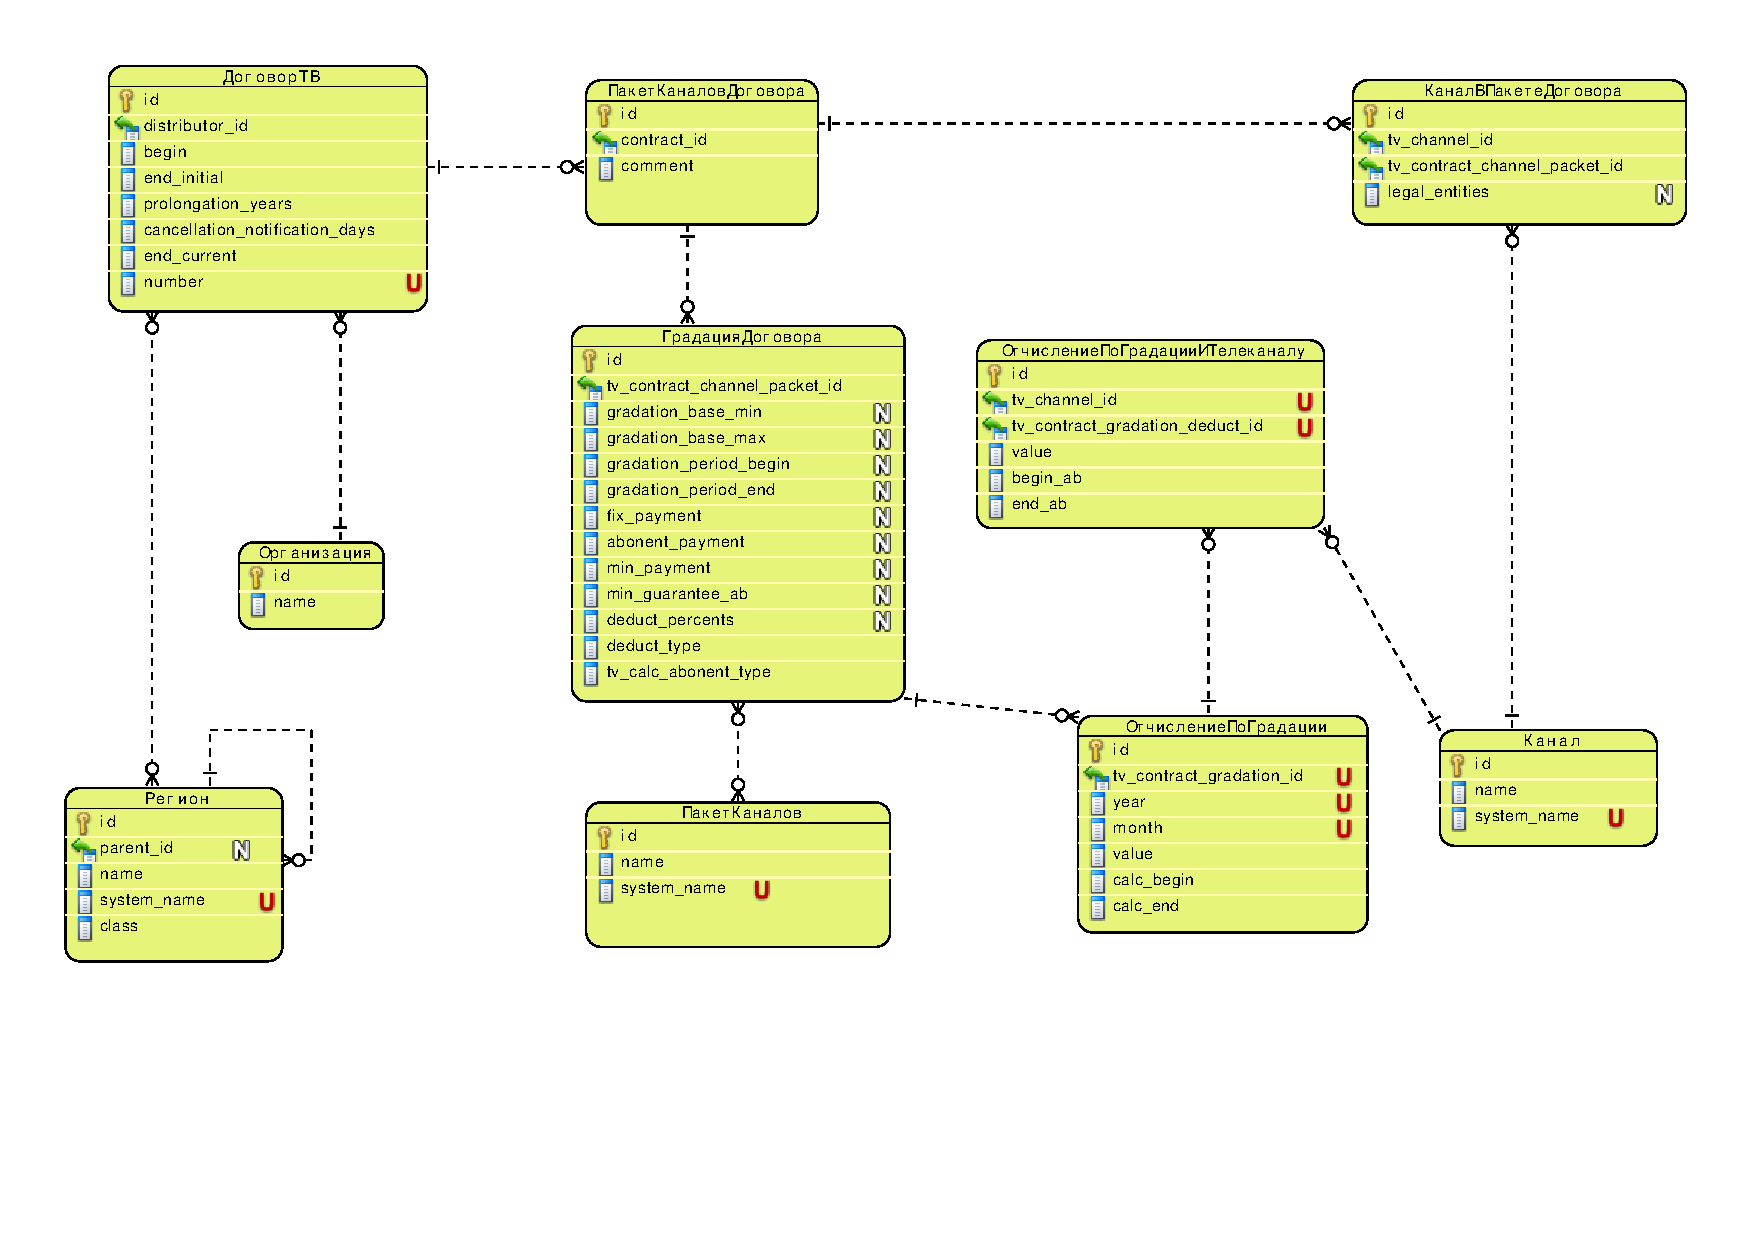
\includegraphics[scale=0.65, trim=10mm 40mm 0mm 10mm, clip]{../resources/uml/TV_DEDUCT.pdf}
\caption{Диаграмма Баркера, демонстрирующая структуру БД для отчислений по Live}
\label{gr:tv_deduct}
\end{center} 
\end{figure}


\paragraph{Справочники} В диаграмме (рис. \ref{gr:tv_deduct}) затронуто описание некоторых справочных
множеств сущностей:
\begin{itemize}
\item{
  \textit{Организация} --- с двумя атрибутами --- идентификатором и названием.
}
\item{
  \textit{Регион} содержит наименование, системное название (в биллинге провайдера), класс территории (тип ENUM),
  и ссылку на родительский регион.
}
\item{
  \textit{Пакет каналов} и \textit{Канал} содержат названия, системные наименования (уникальные идентификаторы).
}
\end{itemize} 

\paragraph{Договоры по Live} В множестве сущностей \textit{ДоговорТВ} отображены договоры по Live, их поля:
\begin{itemize}
\item{
  \textit{distributor\_id} --- внешний ключ, ссылающийся на организацию-правообладатель
}
\item{
  \textit{Номер договора} уникальный номер договора со сквозной нумерацией.
}
\item{
  \textit{Начало действия договора}, \textit{Окончание действия договора (изначальное)}, \textit{Продление срока действия договора (в годах)}
 описывают временной интервал, в котором данный договор является действующим.
}
\end{itemize}

\paragraph{Градации договора} В множестве сущностей \textit{ГрадацияДоговора} отображены градации договоров по Live (см. \ref{live:deducts}), их поля:
\begin{itemize}
\item{
  \textit{gradation\_base\_min, gradation\_base\_max, gradation\_period\_begin, gradation\_period\_end}  
    --- описывают условия применимости градации по базе и по сроку.
}
\item{
  \textit{deduct\_type} и \textit{tv\_calc\_abonent\_type} --- схема расчета и вид расчета базы абонентов градации (тип ENUM).
}
\item{
  \textit{fix\_payment}, \textit{abonent\_payment}, \textit{min\_payment}, \textit{min\_guarantee\_ab},
  \textit{deduct\_percent} --- соответственно ``фиксированный платеж'', ``платеж за абонента'', ``мин.платеж'',
  ``минимальное гарантированное число абонентов'', ``процент отчислений''.
}
\end{itemize}
Следует учитывать, что некоторые из этих полей могут быть незаполненными, что отмечено в диаграмме стереотипом ``N''.

\paragraph{Отчисления по градации} Множество сущностей \textit{ОтчислениеПоГрадации}, которое заполняется 
при расчете отчислений по Live. Сущности, как следует из названия, принадлежат ровно одной градации, соотвественно определен
внешний ключ \textit{tv\_contract\_gradation\_id}.
\begin{itemize}
\item{
  \textit{year} и \textit{month} --- год и номер месяца, для которых был произведен расчет отчислений. 
  Вместе с \textit{tv\_contract\_gradation\_id} составляют потенциальный ключ.
}
\item{
  \textit{calc\_begin} и \textit{calc\_end} --- начало и окончание периода, для которого был произведен расчет отчислений.
  В общем случае могут не соответствовать границе месяца, так как необязательно градация применима для всего месяца.
}
\item{
  \textit{value} --- величина конкретного отчисления (значение в рублях с точностью до $10^{-3}$). 
}
\end{itemize}

\paragraph{Разбивка отчисления} Множество сущностей \textit{ОтчислениеПоГрадацииИТелеканалу}, опреляет величину отчислений
для каждого телеканала пакета градации. 
Каждый объект принадлежит одному из отчислений по градации, а также телеканалу, причем внешние ключи
\textit{tv\_contract\_gradation\_deduct\_id} и \textit{tv\_channel\_id} формируют потенциальный ключ отношения.
\begin{itemize}
\item{
  \textit{begin\_ab} и \textit{end\_ab} --- количество абонентов телеканала на начало и конец периода расчета, 
на основе которого происходил расчет.
}
\item{
  \textit{value} --- величина конкретного отчисления (значение в рублях с точностью до $10^{-3}$). 
}
\end{itemize}

\subsubsection{Статистические данные Live}
\begin{figure}[!ht]
\begin{center}
\vspace{-0.5cm}
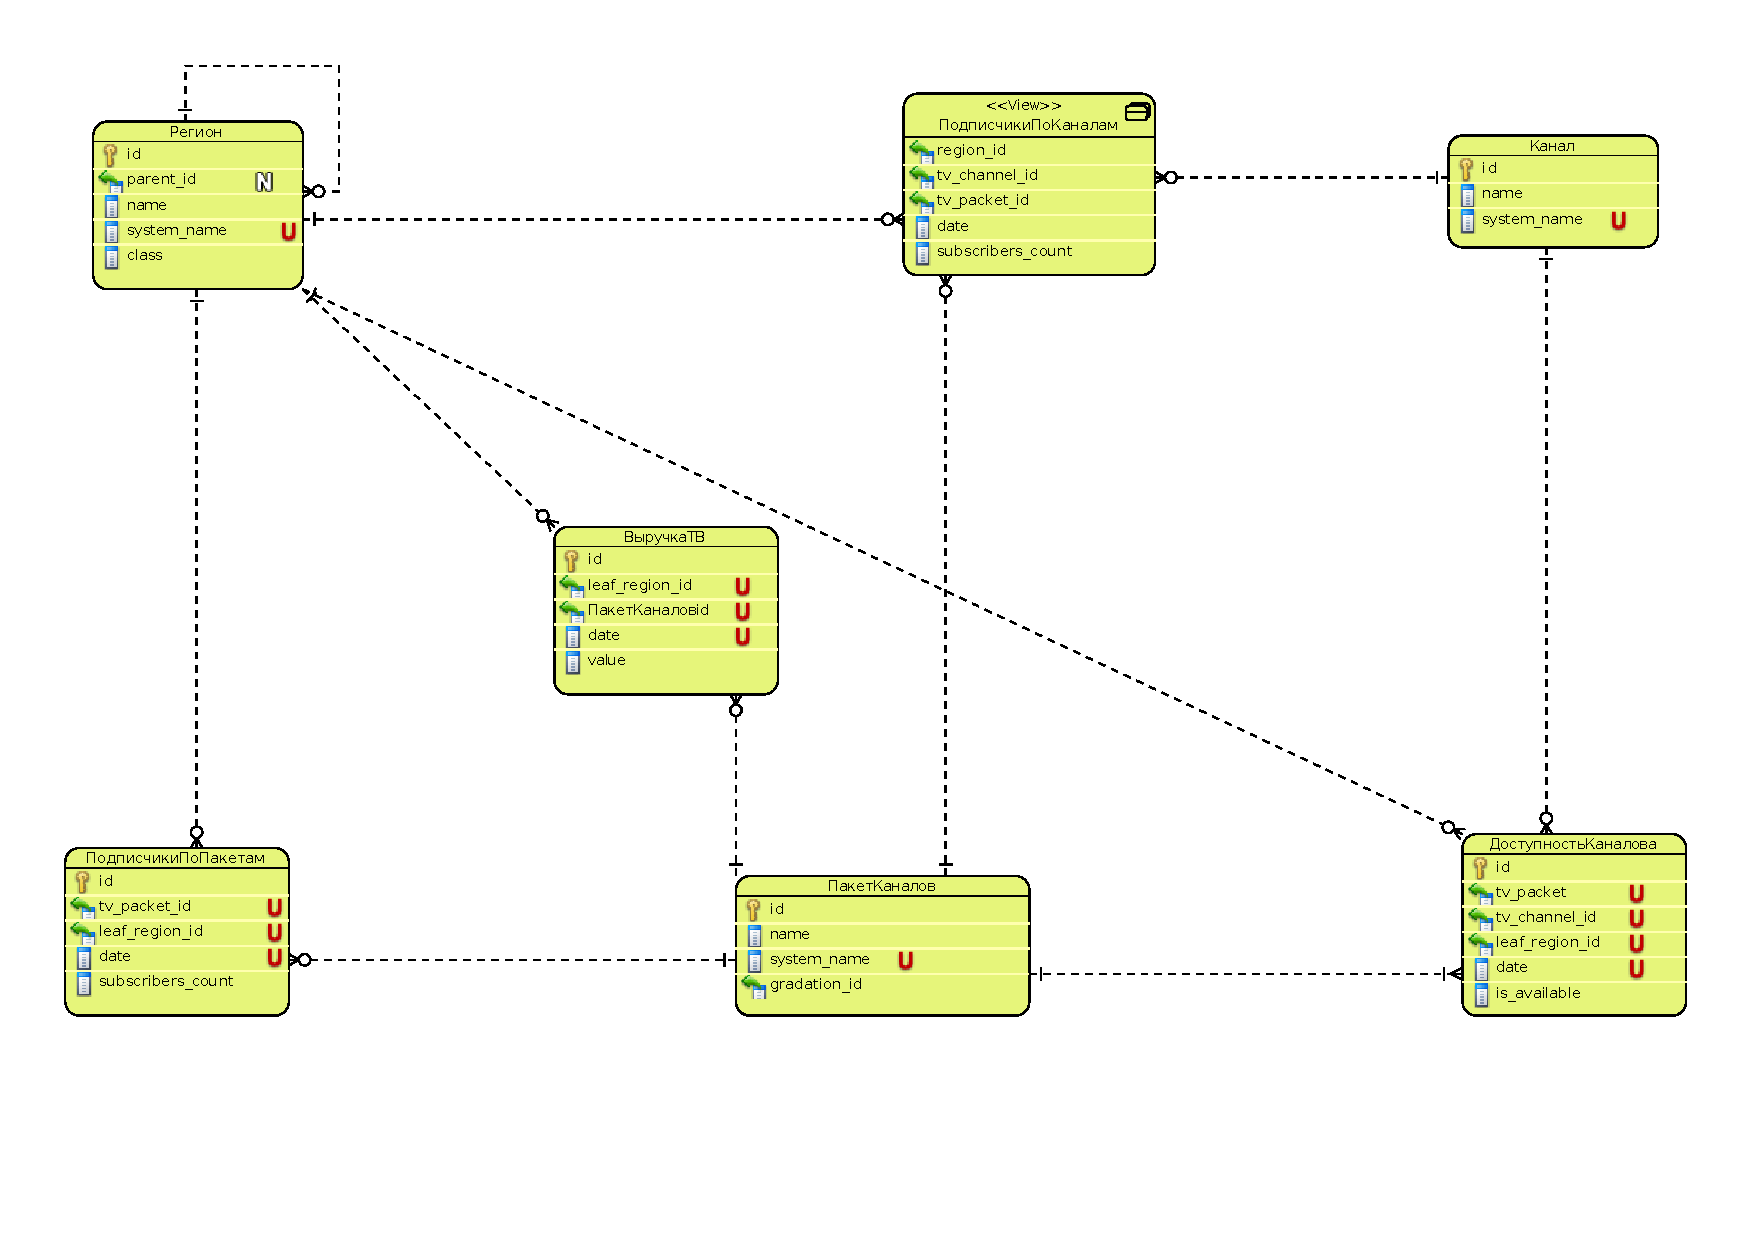
\includegraphics[scale=0.65, trim=10mm 30mm 0mm 10mm, clip]{../resources/uml/TV_STAT.pdf}
\caption{Диаграмма Баркера, демонстрирующая структуру БД для статистических данных по Live}
\label{gr:tv_stat}
\end{center} 
\end{figure}

\paragraph{Абонентская база} Множество сущностей \textit{ПодписчикиПоПакетам} определяет размер
абонентской базы для каждого из пакетов телеканалов в территориях-листьях на каждый день (см. \ref{stat:live}).
\begin{itemize}
\item{
  \textit{tv\_packet\_id} и \textit{leaf\_region\_id} --- внешние ключи для множеств сущностей ``Пакет телеканалов`` и
  ``Регион''.
}
\item{
  \textit{date} --- дата, для которой указано число подсписчков. Вместе со ссылками на пакет и территорию
образует потенциальный ключ.
}
\item{
  \textit{subscribers\_count} --- число подписчиков. 
}
\end{itemize}

\paragraph{Доступность каналов} определяет какие телеканалы были доступны в пакете в определенную дату в пакете для территории.
\begin{itemize}
\item{
  \textit{tv\_packet\_id}, \textit{leaf\_region\_id} и \textit{tv\_channel\_id} --- внешние ключи для множеств сущностей 
``Пакет телеканалов``, ``Регион'' и ``Канал''.
}
\item{
  \textit{date} --- дата, для которой указано число подсписчков. Вместе со ссылками на пакет, территорию и телеканал
образует потенциальный ключ.
}
\item{
  \textit{is\_available} --- параметр доступности, возможные значения --- 0/1. 
}
\end{itemize}

\paragraph{ВыручкаТВ} определяет размер выручки, полученной провайдером для каждого из пакетов телеканалов в территориях-листьях 
за каждый день. Структура аналогична множеству ``ПодписчикиПоПакетам'' за исключением того, что вместо атрибута 
\textit{subscribers\_count} в множестве определен \textit{value}, в котором хранится сумма выручки в рублях с точностью до $10^{-2}$.

\paragraph{ПодписчикиПоКаналам} виртуальное множество сущностей (View), построенное на основе двух других:
``ПодписчикиПоПакетам`` и ``ДоступностьКаналов'', определяющая усредненное число подписчиков по телеканалу в регионе
за определенную дату.

\paragraph{Производительность} Множества сущностей, описанные в этом разделе, при наличии данных за последние пять лет по всем регионам
могут содержать более ста миллионов записей в каждом из них.
В связи с этим было принято решение создать для соотвествующих им таблиц кластерные индексы
с атрибутами ``date'', ``leaf\_region\_id'', ``tv\_packet\_id'', ``tv\_channel\_id''.
Так как в большинстве запросов на выборку данные фильтруются и группируются именно по этим полям
в этом порядке, а также по причине того, что данные будут добавляться именно в хронологическом порядке,
это решение уменьшает, как среднее время добавления объектов, так и время выборки.

\textit{Кластерные индексы} --- один из видов организации индексов в реляционных СУБД, при котором
записи таблицы расположены в файловой системе по возрастанию значения индексируемого множества атрибутов.
В таблице может быть создан только один кластерный индекс. 

\subsubsection{Отчисления по VOD}
\begin{figure}[!ht]

\begin{center}
\vspace{-0.5cm}
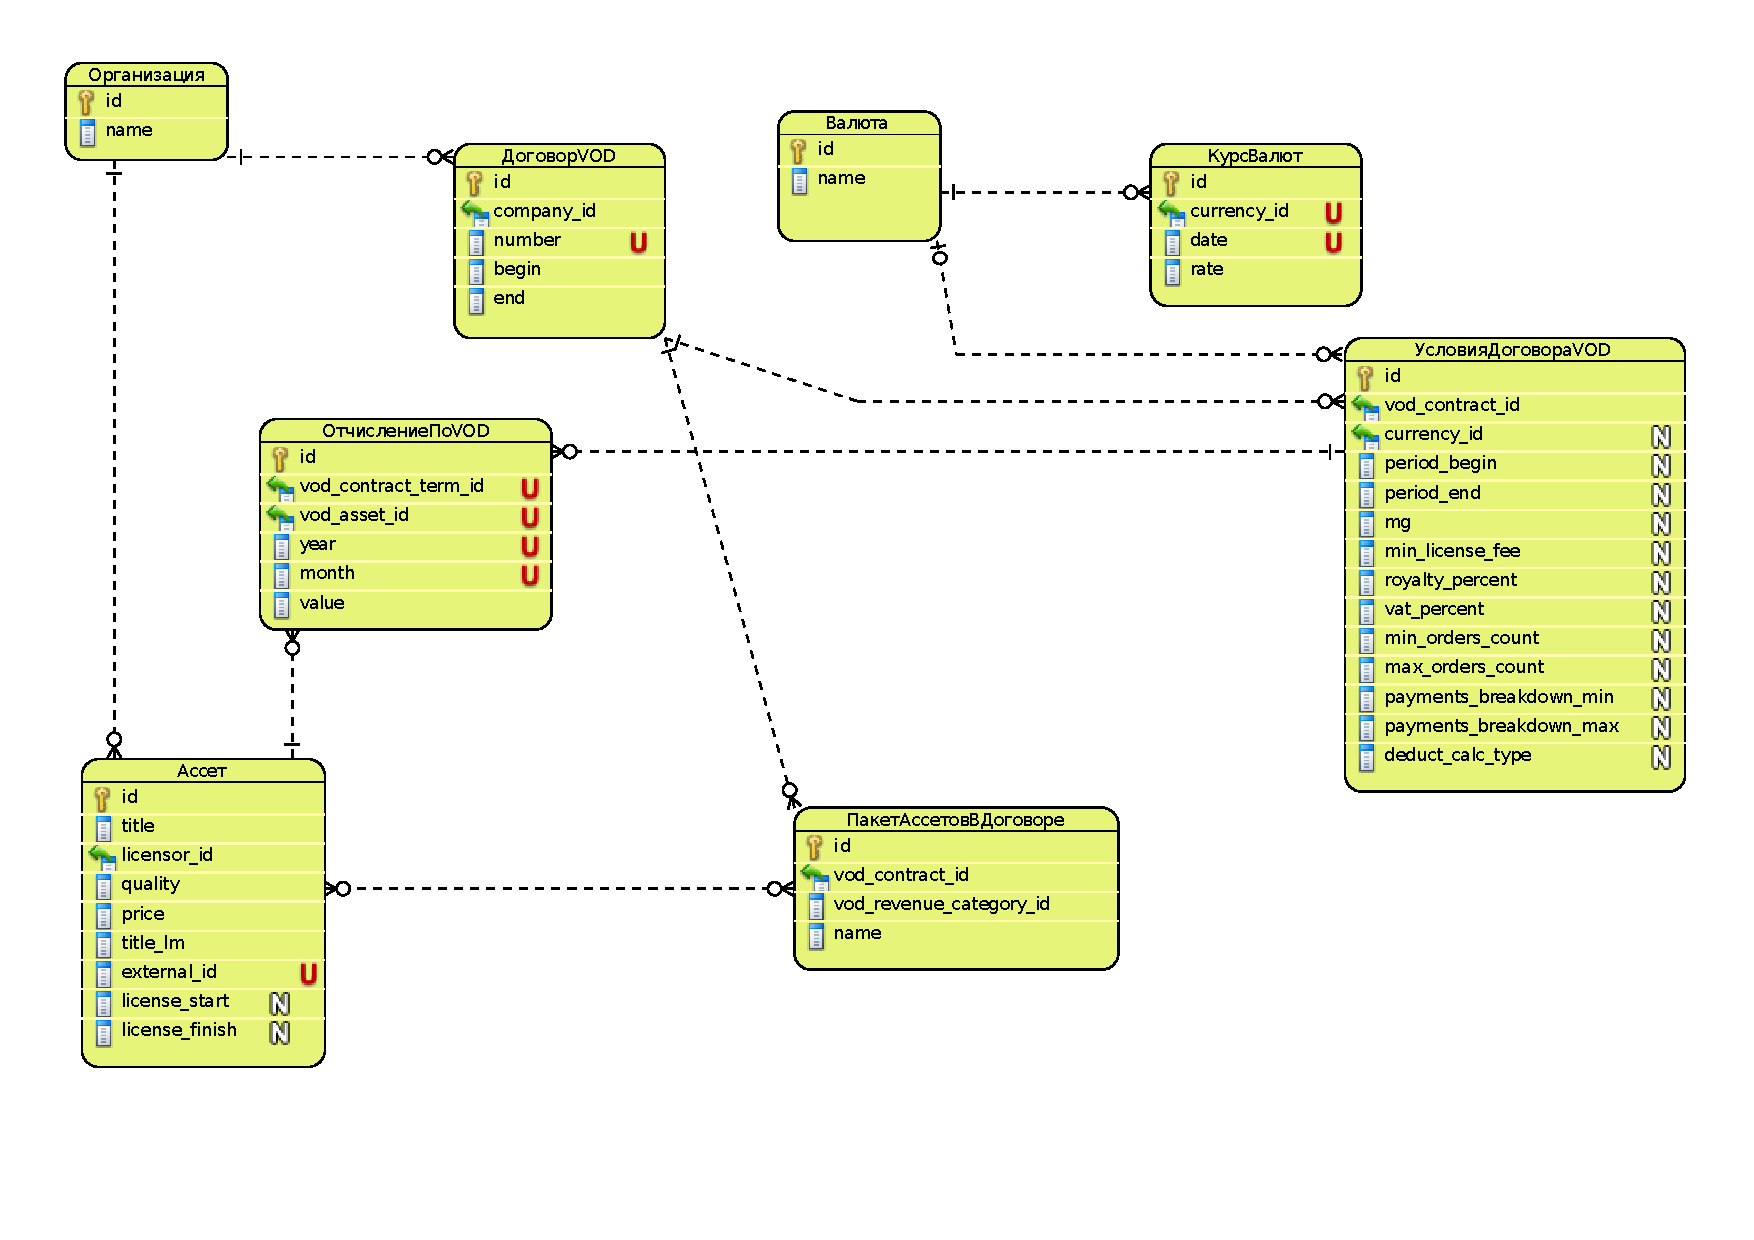
\includegraphics[scale=0.65, trim=10mm 28mm 0mm 10mm, clip]{../resources/uml/VOD_DEDUCT.pdf}
\caption{Диаграмма Баркера, демонстрирующая структуру БД для отчислений по VOD}
\label{gr:vod_deduct}
\end{center} 
\end{figure}

Договоры по VOD (см. \ref{task:contracts}) с их условиями в целом изоморфны договорам по Live с градациями, в связи с этим
подробно рассматривать их структуру не имеет смысла. 

\paragraph{Курсы валют} Так как договоры по VOD могут заключатся в валюте отличной от рублей,
при расчете отчислений необходимо переводить стоимость отчислений в рубли по актуальному курсу.
Для этого в схеме БД добавлены множества сущностей ``Валюта'' и ``КурсВалют''. В множестве
``КурсВалют'' присутствует ссылка на Валюту, вместе с датой эти атрибуты образуют потенциальный ключ.

\paragraph{Ассеты} 
\begin{itemize}
\item{
  \textit{licensor\_id} --- внешний ключ для сущности ``Организация'', для обозначения правообладателя ассета.
}
\item{
  \textit{title} --- название ассета.
}
\item{
  \textit{quality} --- атрибут-показатель качества ассета. Тип ENUM, возможные значения: 3D, SD, HD. 
}
\item{
  \textit{price} --- стоимость заказа по данному ассету на данный момент в рублях.
}
\item{
  \textit{external\_id} --- идентификатор ассета в биллинге провайдера.
}
\item{
  \textit{license\_start} и \textit{license\_finish} --- даты, определяющие срок действия лицензии
провайдера по ассету.
}
\end{itemize}

\newpage

\subsubsection{Статистические данные VOD}
\begin{figure}[!ht]
\begin{center}
\vspace{-0.5cm}
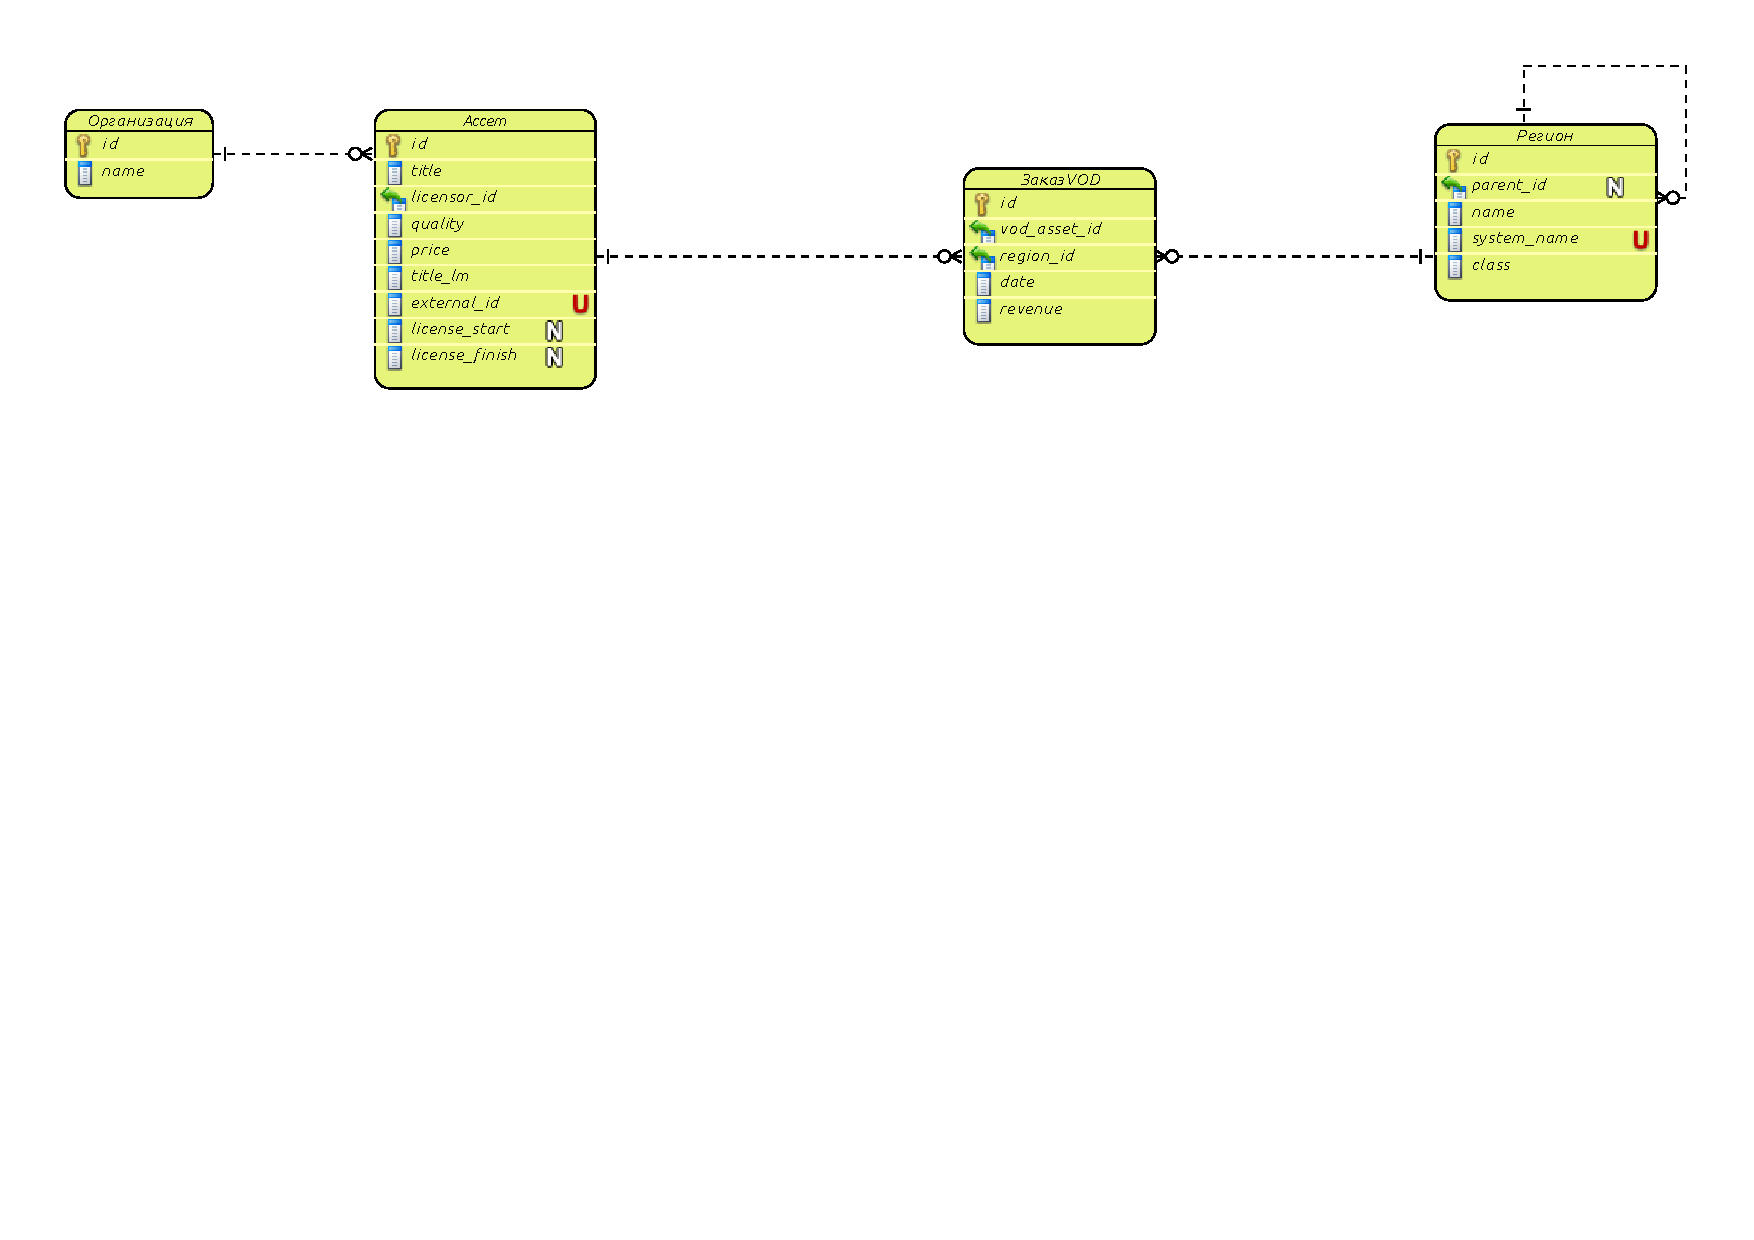
\includegraphics[scale=0.65, trim=10mm 130mm 0mm 10mm, clip]{../resources/uml/VOD_STAT.pdf}
\caption{Диаграмма Баркера, демонстрирующая структуру БД для статистических данных по VOD}
\label{gr:vod_stat}
\end{center} 
\end{figure}

Основной категорией объектов для статистических данных VOD является \textit{ЗаказVOD} (см. \ref{stat:vod}).
Каждый заказ содержит:
\begin{itemize}
\item{
  \textit{vod\_asset\_id} и \textit{region\_id} --- внешние ключи, ссылающиеся на ассет, по которому был сделан
заказ и регион, где находится филиал абонента.
}
\item{
  \textit{date} --- дата, когда был сделан заказ.
}
\item{
  \textit{revenue} --- сумма, которая была заплачена абонентом за заказ в рублях (возможны бесплатные заказы).
}
\end{itemize}
